\documentclass[11pt]{beamer}
\usetheme{Rochester}
\usepackage[utf8]{inputenc}
\usepackage[english]{babel}
\usepackage{amsmath}
\usepackage{amsfonts}
\usepackage{amssymb}
\usepackage{graphicx}
\usepackage{xcolor}
\usepackage{wrapfig}
\usepackage{listings}
\graphicspath{ {./images/} }
\author{Dario Piotrowicz}
\title{Intro to Client-Side Git Hooks (npm specific)}
%\setbeamercovered{transparent} 
%\setbeamertemplate{navigation symbols}{} 
%\logo{} 
%\institute{} 
%\date{} 
%\subject{}
\beamertemplatenavigationsymbolsempty

\AtBeginSection[]{
  \begin{frame}
  \vfill
  \centering
  \begin{beamercolorbox}[sep=8pt,center,shadow=true,rounded=true]{title}
    \usebeamerfont{title}\insertsectionhead\par%
  \end{beamercolorbox}
  \vfill
  \end{frame}
}
 
\begin{document}

\begin{frame}
\titlepage
\end{frame}

\begin{frame}
 \tableofcontents
\end{frame}


\section{Git Hooks}

\begin{frame}{What Git Hooks Are}
  From the
  {\color{purple} \href{https://git-scm.com/docs/githooks\#_description}{official git docs}}:

  \begin{definition}
    Hooks are programs you can place in a hooks directory to trigger actions at certain points in git’s execution. Hooks that don’t have the executable bit set are    ignored.
  \end{definition}
  ~\\
  Hooks are divided in:
  \begin{itemize}
    \item \textbf{Client-Side} \\
  		Hooks executed on the committer's computer
    \item \textbf{Server-Side} \\
        Hooks executed on the server when receiving pushes
  \end{itemize}
  ~\\
  We'll just focus on the client-side here
\end{frame}


\begin{frame}{Client-Side Git Hooks}
  The most important and useful client-side hooks are:
  \begin{itemize}
    \item \textbf{pre-commit} \\
      \begin{tiny}
  		Invoked whem making a commit (before the editor opens for the commit message), it can modify the changes and
  		prevent the commit by exiting with a non-zero value
  		\par
      \end{tiny}
    \item \textbf{pre-push} \\
      \begin{tiny}
       Invoked when pushing to remote, can be used to perform checks (by the way, the remote destination is provided as parameter to
       the hook) and prevent the push by exiting with a non-zero value
       \par
      \end{tiny}
    \item \textbf{commit-msg} \\
	  \begin{tiny}
       Invoked when committing or merging, it receives the name of the file that holds the proposed commit log message and can modify it,
       can also prevent the commit/merge by exiting with a non-zero value
       \par
      \end{tiny}
    \item \textbf{prepare-commit-msg} \\
      \begin{tiny}
        Invoked when commiting, it's purpose is to edit the default commit message that is proposed to the committer,
        just like the others can abort the commit by exiting with a non-zero value 
        \par
      \end{tiny}
  \end{itemize}
  ~\\
  You can find the list of all the git hooks supported in the
  {\color{purple} \href{https://git-scm.com/docs/githooks\#_hooks}{official git docs}}
\end{frame}






\section{Tools}


\begin{frame}{Husky}
  \begin{wrapfigure}{0}{0.125\textwidth}
    \vspace*{-2em}
    \centering
    
\includegraphics[width=0.125\textwidth]{husky.png}
  \end{wrapfigure}

  One of the most popular ways to implement\\
  git hooks is by using {\color{purple} \href{https://typicode.github.io/husky}{husky}}
  \\~\\
  But:
  \begin{itemize}
    \item \textbf{Husky v.4 adds overhead and has dependencies} \\
      \begin{scriptsize}
  		Based on it's implementation there are extra checks and overheads than necessary
  		\par
           \end{scriptsize}
    \item \textbf{Husky v.5 has a Parity License} \\
      \begin{scriptsize}
        Later the license should change to MIT, but currently uses the {\color{purple} \href{https://paritylicense.com/}{Parity License}}
        preventing its usage in non open source projects
        \par
      \end{scriptsize}
    \item \textbf{Is Unnecessary} \\
	  \begin{scriptsize}
       Both v.4 and v.5 are quite unnecessary, everything they do can be done with practically the same effort natively
       \par
      \end{scriptsize}
  \end{itemize}
  ~\\
  So...
\end{frame}


\begin{frame}{Native Git Hooks}
  Writing git hooks in the native way is very easy and doesn't have drawbacks
  \\~\\
  For that all you need to do is writing a script file which name corresponds to the hook that you're implementing and add it to the project's hook directory
  \\~\\
  Let's just see how it is done with an example, let's implement the \textbf{pre-commit} hook
\end{frame}



\begin{frame}[fragile]{Native Git Hooks - pre-commit 1}
  We can just create this file:
    \begin{lstlisting}[frame=single,columns=fullflexible]
   #!/bin/sh
   echo "Hello World of Hooks";
   \end{lstlisting}
  ~\\
  Make it executable, place it in the \textbf{.git/hooks} directory of our project and that is actually it!
  \\~\\
  If we now try to commit some code we will just be presented with the \textit{Hello World of Hooks} line (and everything will keep working as normal)
  \\~\\
  Is this enough? can you spot a problem with this approach?
\end{frame}


\begin{frame}[fragile]{Native Git Hooks - pre-commit 2}
 There's a significant problem here, the \textbf{.git} directory is external from the git flow and doesn't get committed, so basically this hook will only work on your  personal machine and no one pulling down will notice anything different
 \\~\\
 The solution is simply to move the hook in a directory which will git will keep track of like for example a \textbf{git-hooks} directory
 \\~\\
 But now we do need to tell git to consider this one the new directory containing our project's hooks and we can do it with:
 \begin{lstlisting}[columns=fullflexible]
   git config core.hooksPath ./git-hooks
 \end{lstlisting}
\end{frame}



\begin{frame}[fragile]{Native Git Hooks - pre-commit 2}
  This is ok and the hooks will be part of the repository, but in order for the committer to use them they will have to run the config command
  \\~\\
  So let's add a new script to out \textit{package.json} so that this will be done automatically after every installation:
  \begin{footnotesize}
    \begin{lstlisting}[frame=single,columns=fullflexible]
 scripts: {
   ...,
   postinstall: "git config core.hooksPath ./git-hooks",
   ...
 }
   \end{lstlisting}
  \end{footnotesize}
  ~\\
  Now everything is fine and as soon as a committer pulls down the code and runs `npm install` the hooks will be set for them 
\end{frame}






\section{Examples}



\begin{frame}{Using the Pre-commit hook with Prettier}
  A popular use of the pre-commit hook is to format your code using prettier when commits are made
  \\~\\
  Prettier also does specifies this in its {\color{purple} \href{https://prettier.io/docs/en/precommit.html}{official docs}}
  \\~\\
  Tools such as 
  {\color{purple} \href{https://github.com/azz/pretty-quick}{pretty-quick}}
  and
  {\color{purple} \href{https://github.com/okonet/lint-staged}{lint-staged}}
  are very popular and allow you to format and lint only staged files with close to no effort
\end{frame}



\begin{frame}{Angular's Commit Message Format}
  The Angular repo requires a
  {\color{purple} \href{https://github.com/angular/angular/blob/master/CONTRIBUTING.md\#commit}{specific commit message format}}
  \\~\\
  In order to ``enforce'' it they have a (husky) \textbf{commit-msg} set up as you can see here: 

  \begin{center}
   \href{https://github.com/angular/angular/blob/master/.husky/commit-msg}{
      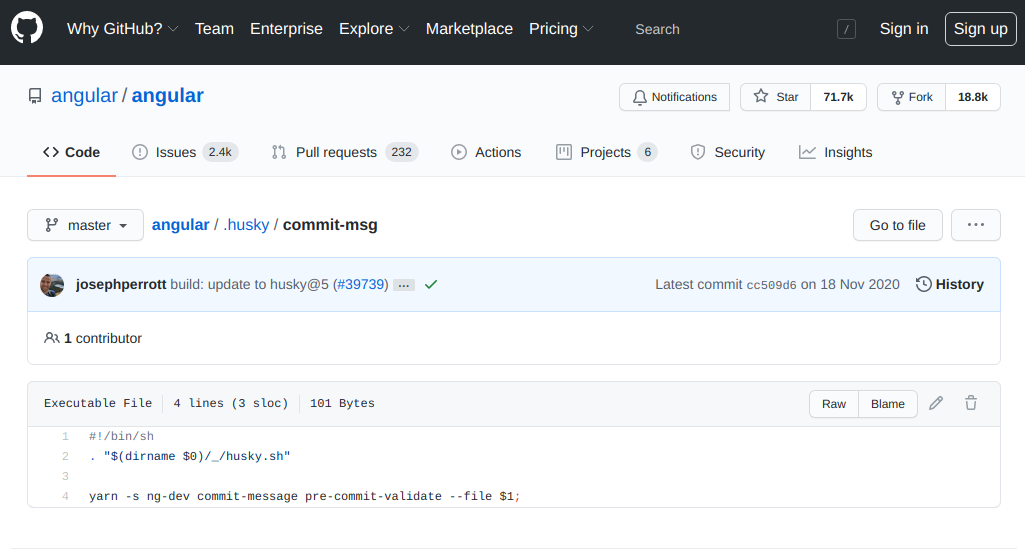
\includegraphics[scale=0.2]{angular-commit-msg.png}
   }
  \end{center}
\end{frame}



\begin{frame}{React's pre-commit linting hook}
  React has a \textbf{pre-commit} hook to eslint the staged \textit{js} files
  \begin{center}
   \href{https://github.com/facebook/react/blob/master/scripts/git/pre-commit}{
      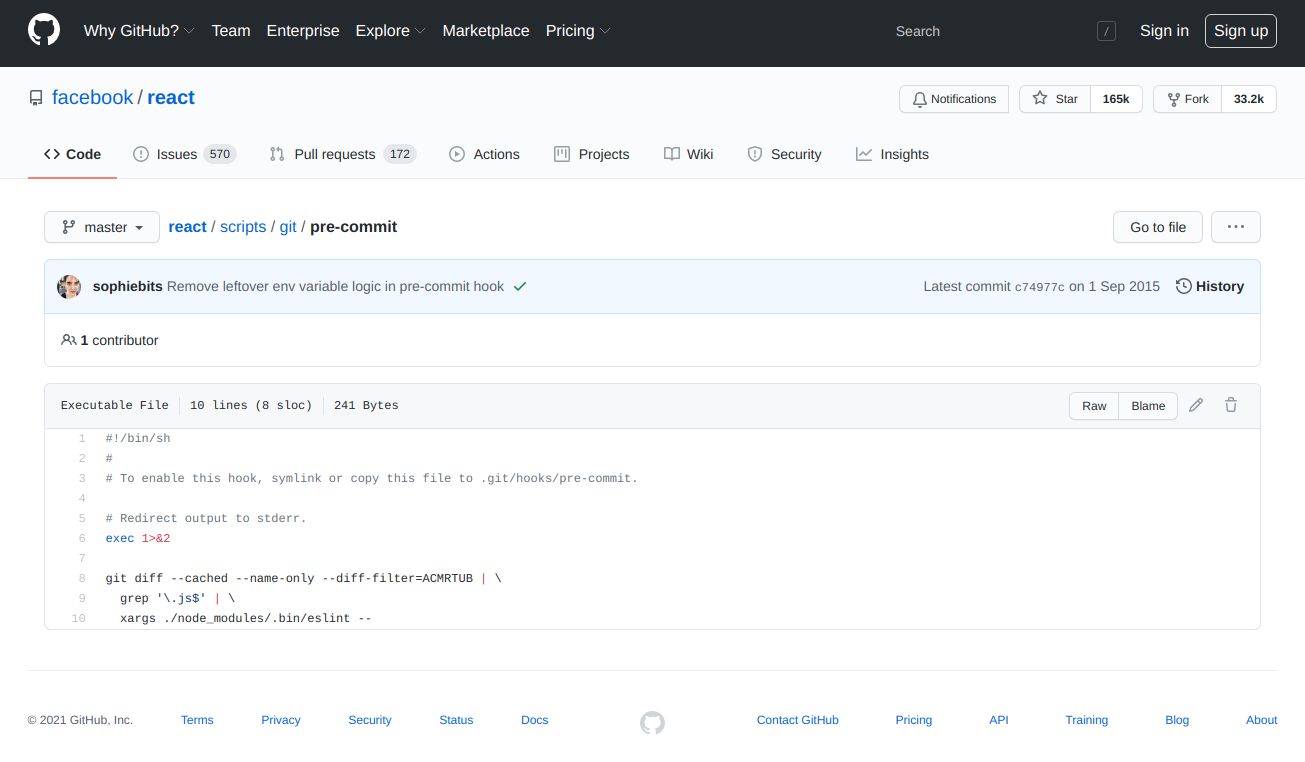
\includegraphics[scale=0.2]{react-pre-commit.png}
   }
  \end{center}
\end{frame}


\begin{frame}{Vue's package.json gitHooks}
  The Vue repo implements both a \textbf{pre-commit} and \textbf{commit-msg} in its package.json using a fork of husky v4 (called
  {\color{purple} \href{https://github.com/yyx990803/yorkie}{yorkie}}):

  \begin{center}
   \href{https://github.com/vuejs/vue/blob/dev/package.json\#L46}{
      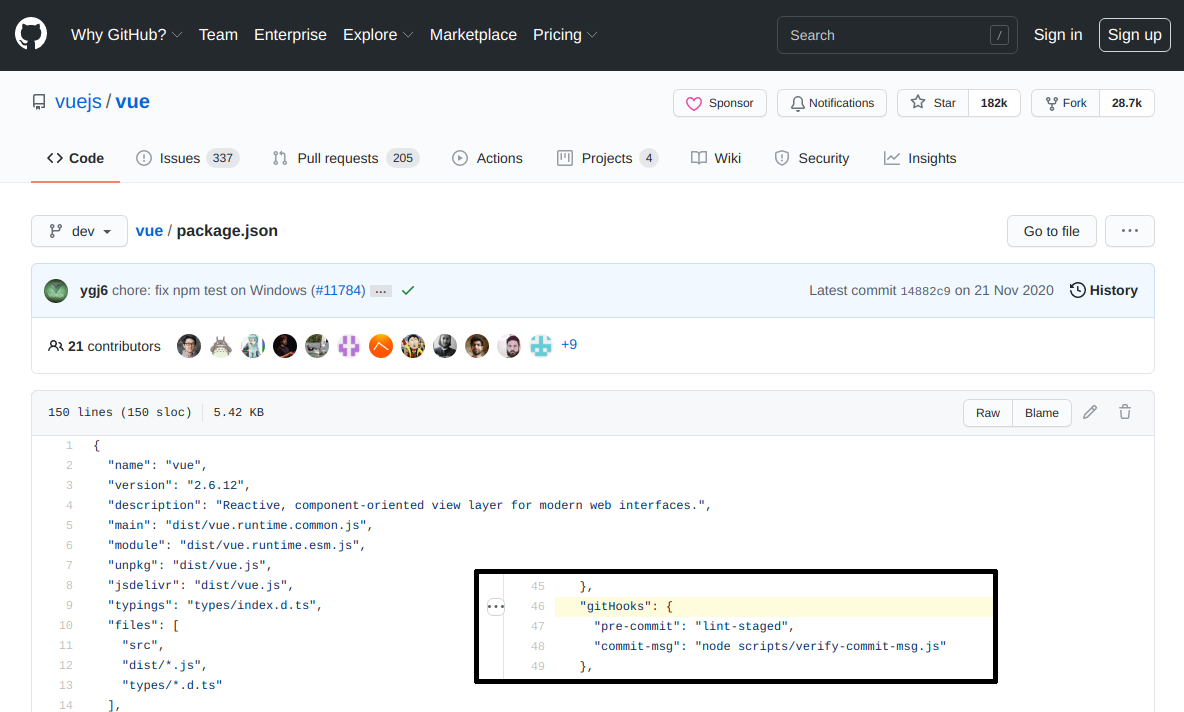
\includegraphics[scale=0.2]{vue-githooks.png}
   }
  \end{center}
\end{frame}


\end{document}